\documentclass{article}
\usepackage[T1]{fontenc}
\usepackage[utf8]{inputenc}
\usepackage{ismir}
\usepackage{amsmath,cite,url}
\usepackage{graphicx}
\usepackage{booktabs}
\newcommand{\NTempo}{290}
\newcommand{\AccOneAC}{39.3}
\newcommand{\AccTwoAC}{87.2}
\newcommand{\AccOnePulse}{19.0}
\newcommand{\AccTwoPulse}{76.2}
\newcommand{\AccOnePrior}{66.6}
\newcommand{\AccTwoPrior}{89.7}
\newcommand{\AccOneIOI}{47.6}
\newcommand{\AccTwoIOI}{85.9}
\newcommand{\AccOneLibrosa}{70.7}
\newcommand{\AccTwoLibrosa}{87.2}
\newcommand{\AccOneMadmom}{81.4}
\newcommand{\AccTwoMadmom}{96.9}
\newcommand{\HalfAC}{34.5}
\newcommand{\MadmomMs}{2.1}
\newcommand{\LibrosaMs}{46}
\newcommand{\AccOneStretchMin}{67.2}
\newcommand{\AccOneStretchMax}{74.1}
\newcommand{\RelErrFour}{1.7}
\newcommand{\RelErrTwelve}{1.1}
\newcommand{\SpliceMAE}{18.7}
\newcommand{\SettleMed}{0.3}
\newcommand{\SettleFrac}{62}
\newcommand{\NChange}{58}
\newcommand{\DetFoldMed}{1.2}
\newcommand{\DetFoldTwo}{75}
\newcommand{\DetRawMed}{2.2}
\newcommand{\DetRawTwo}{46}
\newcommand{\BestTight}{300}
\newcommand{\DPF}{0.76}
\newcommand{\DPCML}{0.57}
\newcommand{\DPAML}{0.85}
\newcommand{\DPOracleF}{0.84}
\newcommand{\DPOracleCML}{0.85}
\newcommand{\DPOracleAML}{0.89}
\newcommand{\LibF}{0.76}
\newcommand{\LibCML}{0.62}
\newcommand{\LibAML}{0.81}
\newcommand{\MadF}{0.88}
\newcommand{\MadCML}{0.79}
\newcommand{\MadAML}{0.94}
\newcommand{\NNF}{0.64}
\newcommand{\NNCML}{0.23}
\newcommand{\NNAML}{0.47}
\newcommand{\NNDBNF}{0.83}
\newcommand{\NNDBNCML}{0.71}
\newcommand{\NNDBNAML}{0.88}
\newcommand{\NBeat}{290}
\newcommand{\AgreeMed}{0.98}
\newcommand{\AgreeShare}{74}
\newcommand{\AgreeRawMed}{0.96}
\newcommand{\LibBeatTime}{0.23}
\newcommand{\MadTime}{6.4}
\newcommand{\NNDBNTime}{0.51}
\newcommand{\MLPTime}{0.39}
\newcommand{\DPTime}{0.35}
\newcommand{\DegClean}{0.79}
\newcommand{\DegOrClean}{0.89}
\newcommand{\PercClean}{0.80}
\newcommand{\MadDegClean}{0.90}
\newcommand{\DegNoiseZero}{0.80}
\newcommand{\DegOrNoiseZero}{0.91}
\newcommand{\PercNoiseZero}{0.78}
\newcommand{\MadDegNoiseZero}{0.90}
\newcommand{\DegNoiseMinusTen}{0.60}
\newcommand{\DegOrNoiseMinusTen}{0.75}
\newcommand{\PercNoiseMinusTen}{0.53}
\newcommand{\MadDegNoiseMinusTen}{0.68}
\newcommand{\DegWhite}{0.79}
\newcommand{\DegOrWhite}{0.90}
\newcommand{\PercWhite}{0.78}
\newcommand{\MadDegWhite}{0.88}
\newcommand{\DegLPOne}{0.75}
\newcommand{\DegOrLPOne}{0.86}
\newcommand{\PercLPOne}{0.73}
\newcommand{\MadDegLPOne}{0.85}
\newcommand{\DegLPFour}{0.78}
\newcommand{\DegOrLPFour}{0.88}
\newcommand{\PercLPFour}{0.78}
\newcommand{\MadDegLPFour}{0.90}
\newcommand{\DegMPThree}{0.79}
\newcommand{\DegOrMPThree}{0.88}
\newcommand{\PercMPThree}{0.80}
\newcommand{\MadDegMPThree}{0.90}
\newcommand{\NDeg}{58}
\newcommand{\DBOracle}{0.34}
\newcommand{\NDown}{290}
\newcommand{\DBFirst}{0.26}
\newcommand{\DBNN}{0.17}
\newcommand{\DBNNFirst}{0.17}
\newcommand{\DBMadJoint}{0.65}
\newcommand{\DBMadBar}{0.76}

%% method paragraphs, one macro per member, reused by all three reports
\newcommand{\MethodIrai}{%
\textbf{Autocorrelation tempo estimation (Irai).} The autocorrelation
\begin{equation}
r(\tau) = \sum_n o(n)\,o(n+\tau)
\end{equation}
is computed with the FFT, and the plain estimate is $\hat{T} = 60 f_r/\tau^\ast$ for the lag $\tau^\ast$ with the largest $r(\tau)$ between 40 and 250\,BPM. A pulse train stage following \cite{percival} scores the ten strongest autocorrelation peaks by the best phase-aligned match of pulses at $\tau$, $1.5\tau$ and $2\tau$. The octave decision stage weights each of the ten candidates $\hat{T}_k$ by a log-normal prior,
\begin{equation}
s_k = r(\tau_k)\, \exp\!\Big(-\tfrac{1}{2}\log_2^2 \frac{\hat{T}_k}{120}\Big),
\label{eq:prior}
\end{equation}
and returns the candidate with the largest $s_k$. An inter-onset-interval (IOI) histogram of picked onsets is a simple baseline. For Objective 2, clips are time-stretched with the ffmpeg \texttt{atempo} filter, which keeps the pitch, so the true tempo becomes $fT$ for a factor $f$. The local estimator applies the octave decision to sliding windows of length $W$ with a hop of 1\,s. Spliced clips join a part stretched by $f_1$ to a part stretched by $f_2$ with a 10\,ms crossfade, at 15\,s of the source for the tracking test and at a random point between 10 and 20\,s for the detection test, in both directions. The change detector folds the local tempo curve into one octave around its median, $u_i = \mathrm{wrap}(\log_2(\hat{T}_i/\mathrm{med}\,\hat{T}))$ with $\mathrm{wrap}$ to $[-\tfrac12, \tfrac12)$, so that octave jumps do not look like changes, and picks the split point that minimises the squared deviation of $u$ from the median of each side.}

\newcommand{\MethodNalluraj}{%
\textbf{Dynamic programming beat tracking (Nalluraj).} Following Ellis \cite{ellis}, the tempo is estimated from the autocorrelation of $o(n)$ weighted by a log-Gaussian window around 120\,BPM, giving a beat period $p$ in frames. The best score of a beat sequence ending at frame $t$ is
\begin{equation}
C(t) = o(t) + \max_{\tau \in [t-2p,\, t-p/2]} \Big( C(\tau) - \alpha \log^2\!\frac{t-\tau}{p} \Big),
\label{eq:dp}
\end{equation}
where the tightness $\alpha$ sets how strongly the tracker keeps an even spacing. The beat sequence is recovered by backtracking from the best frame near the end. The tracker is run with the estimated tempo and with the oracle tempo from the annotations, which separates tempo errors from beat placement errors. For Objective 2, clips are degraded with pink noise at 20 to $-10$\,dB SNR, white noise at 0\,dB, a sixth-order zero-phase Butterworth low pass filter at 4, 2 and 1\,kHz, and MP3 encoding at 128, 64 and 32\,kbps with ffmpeg. The percussive envelope applies the same spectral flux to the percussive part of a median-filter harmonic-percussive separation (17-frame kernels).}

\newcommand{\MethodUsha}{%
\textbf{Neural network beat tracking (Usha).} Each frame is described by its 40 log-mel values and their positive differences, normalised per clip and stacked over $\pm 4$ frames (720 features). A multilayer perceptron (MLP) with two hidden layers of 128 and 64 units predicts the probability $a(n)$ that frame $n$ lies within one frame of a beat. Negative frames are subsampled to three times the positive frames, and training stops early on a 10\% validation part. Beats are the peaks of the smoothed activation that exceed a local mean by 0.05 and are at least 0.2\,s apart. As a second decoder, $a(n)$ is passed to madmom's DBN beat tracker \cite{madmom, downbeat}, which only uses our activation and no madmom network.

\textbf{Downbeat finder (Usha).} Given beats $b_1, \dots, b_K$ and a bar length $L$ from the annotations, the finder takes the peak of the low-frequency onset envelope $o_{\mathrm{low}}$ (six lowest mel bands, below about 200\,Hz) within 50\,ms of each beat and chooses the bar phase
\begin{equation}
\phi^\ast = \arg\max_{\phi \in \{0,\dots,L-1\}} \frac{1}{|\{k : k \equiv \phi\}|}\sum_{k \equiv \phi \,(\mathrm{mod}\, L)} o_{\mathrm{low}}(b_k),
\label{eq:down}
\end{equation}
on the idea that the kick drum and bass mark the downbeat. A baseline takes the first beat as the downbeat.}

\newcommand{\PITable}{%
\begin{table}[t]
\centering\small\setlength{\tabcolsep}{5pt}
\begin{tabular}{@{}llccccc@{}}
\toprule
Member & Obj. & PI1 & PI2 & PI3 & PI4 & PI5 \\
\midrule
Irai & 1 & D & P & D$^\ast$ & D & D \\
Irai & 2 & D & D & D & D & D \\
Nalluraj & 1 & D & D & D & D & -- \\
Nalluraj & 2 & D & D & P & D & -- \\
Usha & 1 & D & P & D & P & -- \\
Usha & 2 & D & D & D & D & -- \\
\bottomrule
\end{tabular}
\caption{Status of all performance indicators. D: done, P: partly done, --: not started. PI1 and PI2 are basic, PI3 and PI4 expected, PI5 advanced. $^\ast$Done, with a negative result.}
\label{tab:pi}
\end{table}}

\newcommand{\TimelineTable}{%
\begin{table}[t]
\centering\small\setlength{\tabcolsep}{3pt}
\begin{tabular}{@{}lp{0.80\columnwidth}@{}}
\toprule
Week & Plan (status) \\
\midrule
1--2 & Spec, repository, data, shared front end, basic methods (done) \\
3--4 & Evaluation on GTZAN, librosa and madmom comparisons (done) \\
5 & TCN in PyTorch (Usha); 1D State Space tracker under the same tests (Nalluraj, Usha); GiantSteps tempo (Irai) \\
6 & Advanced goals: tempo following and automatic tightness (Nalluraj), TCN with downbeat output and stretch augmentation (Usha), pulse train fix and change detection on real tempo changes (Irai) \\
7 & Final report and presentation (Dec 1--7) \\
\bottomrule
\end{tabular}
\caption{Revised timeline. Weeks 5 and 6 are Nov 17--23 and Nov 24--30.}
\label{tab:time}
\end{table}}

\newcommand{\MeIntro}{This report is Nalluraj's individual submission: Section~\ref{sec:me} is his status report, and Section~\ref{sec:team} summarises the rest of the group.}

\title{Dynamic Programming Beat Tracking on Degraded Audio: Progress Report}

\threeauthors
  {Nalluraj Babu}{University of Victoria}
  {Irai Kumaran Sivanesan}{University of Victoria}
  {Usha Sundaresan Manivannan}{University of Victoria}

\sloppy
\begin{document}
\maketitle

\begin{abstract}
This is the progress report of Nalluraj Babu for the CSC 475/575 group project DP2\_B on tempo estimation and beat tracking. My part is a dynamic programming beat tracker following Ellis, built from scratch, and a study of beat tracking on degraded audio. On the artist-filtered GTZAN test split (\NBeat{} clips) the tracker reaches a mean F-measure of \DPF{} with its own tempo estimate and \DPOracleF{} with the annotated tempo, the same accuracy as librosa (\LibF{}) and below madmom (\MadF{}). Across 13 degradations the tracker is robust to MP3 compression and moderate noise, but loses accuracy with a 1\,kHz low pass filter and with pink noise at $-10$\,dB SNR; madmom degrades in a similar way from a higher level. I also report the status of my teammates and our revised plan.
\end{abstract}

\section{Introduction}

Tempo estimation finds how fast a piece of music is, in beats per minute (BPM), and beat tracking finds the times at which a listener would tap along. Both are basic tasks in music information retrieval and a first step for downbeat tracking, chord recognition and structure analysis \cite{tutorial}. Our group (Default Project 2, DP2\_B) set three goals in the design specification: build one complete method per member from scratch, compare these methods with existing tools, and study three known weak spots: changing tempo, degraded audio and the bar level (downbeats).

Each member owns one method and one study. Irai Kumaran Sivanesan works on tempo estimation and tempo changes, Nalluraj Babu on dynamic programming beat tracking and degraded audio, and Usha Sundaresan Manivannan on neural network beat tracking and downbeats. \MeIntro{} All code, result files and the scripts that make every number, table and figure in this report are in our repository.\footnote{\url{https://github.com/Iraikumaran/beat-tracking}, branch \texttt{Dev}.}

\section{Related Work}

Most tempo and beat systems first compute an onset detection function \cite{bello} and then look for periodicities in it. Gouyon et al. \cite{gouyon} compared tempo induction algorithms, introduced the Accuracy1 and Accuracy2 measures, and showed that choosing half or double the correct tempo is the most common error. Percival and Tzanetakis \cite{percival} proposed a streamlined estimator based on autocorrelation followed by cross-correlation with pulse trains. Ellis \cite{ellis} framed beat tracking as dynamic programming over an onset envelope, the method behind the beat tracker of librosa \cite{librosa}. For music with changing tempo, Grosche and M\"uller \cite{plp} estimate a local pulse in short windows.

Neural networks now give the best results. B\"ock et al. \cite{downbeat} predict beat and downbeat activations with recurrent networks and decode them with a dynamic Bayesian network (DBN), as implemented in madmom \cite{madmom}. Krebs et al. \cite{krebsbar} find downbeats from beat-synchronous features. Davies and B\"ock \cite{tcn} showed that temporal convolutional networks (TCNs) are accurate and small, and Heydari et al. \cite{heydari} reduced decoding cost with a one dimensional state space. Davies et al. \cite{tutorial} give a practical overview of all of these methods. Mauch and Ewert \cite{degradation} showed that MIR systems, beat trackers included, lose accuracy under common audio degradations.

Evaluation follows Davies et al. \cite{daviseval} with the reference implementation in mir\_eval \cite{mireval}. GTZAN was introduced by Tzanetakis and Cook \cite{gtzan}; Sturm \cite{sturm} documents its faults, and Kereliuk et al. \cite{kereliuk} proposed the artist-filtered split we use. The beat and downbeat annotations come from Marchand et al. \cite{marchand}. GiantSteps Tempo \cite{giantsteps} is the second dataset in our plan.

\section{Data and Evaluation}

We use the GTZAN audio with the beat, downbeat and tempo annotations of the gtzan\_tempo\_beat repository \cite{tutorial, marchand}. All results are on the artist-filtered test split of Kereliuk et al. \cite{kereliuk} (\NTempo{} clips of 30\,s, all ten genres). The neural network is trained on 160 clips from the matching training and validation splits (16 per genre), so no test artist is seen in training. The studies on tempo changes and degraded audio use an evenly spaced subset of \NDeg{} test clips (every fifth clip, all genres). The reference tempo of a clip is $T = 60/\mathrm{median}(\Delta b)$, where $\Delta b$ are the annotated inter-beat intervals.

For a tempo estimate $\hat{T}$, Accuracy1 counts $|\hat{T}-T| \le 0.04\,T$, and Accuracy2 also accepts $\hat{T}$ within 4\% of $kT$ for $k \in \{2, 3, \tfrac{1}{2}, \tfrac{1}{3}\}$. For beats and downbeats we report the F-measure with a $\pm 70$\,ms tolerance window,
\begin{equation}
F = \frac{2PR}{P+R},
\end{equation}
where $P$ and $R$ are the precision and recall of the estimated beats, together with the continuity measures CMLt and AMLt \cite{daviseval}. CMLt asks for a continuous sequence at the correct metrical level, and AMLt also accepts double, half and off-beat sequences. Beats in the first 5\,s are ignored; for downbeats they are kept.

\textbf{Shared front end.} Audio is resampled to 22.05\,kHz and a short-time Fourier transform is computed with a 2048-sample Hann window and a hop of 256 samples ($f_r = 86.1$ frames per second). The magnitude is mapped to 40 mel bands and compressed as $M(f,n) = \log(1 + 100\,X_{\mathrm{mel}}(f,n))$. The onset envelope is the half-wave rectified spectral flux
\begin{equation}
o(n) = \sum_f \max\big(0, M(f,n) - M(f,n-1)\big),
\end{equation}
with a moving average removed and the result normalised. Our own methods use only NumPy, SciPy and scikit-learn; librosa \cite{librosa} and madmom \cite{madmom} are used only as reference systems.

\textbf{Repeatability.} Every experiment was run twice from a clean results folder on the same machine. Apart from run times, the two runs gave identical result files, and they also matched the files that each member had produced on their own laptop (two of 6090 rows in the tightness sweep differ, both at $\alpha = 3000$, by floating point effects).


\section{Methods}
\label{sec:methods}

\MethodNalluraj

\textbf{Reference systems.} librosa's \texttt{beat\_track} implements the same algorithm with its own onset envelope and tempo estimate. madmom combines a recurrent network that predicts beat activations with a DBN decoder \cite{downbeat, madmom}. To check our implementation, both trackers were also given librosa's onset envelope and tempo, and their beat sequences were compared with the F-measure.

\begin{table}[t]
\centering\small\setlength{\tabcolsep}{4pt}
\begin{tabular}{@{}lccc@{}}
\toprule
Beat tracker & F & CMLt & AMLt \\
\midrule
\csname @@input\endcsname ../figures/tab_beats.tex
\bottomrule
\end{tabular}
\caption{Beat tracking on the GTZAN test split (\NBeat{} clips). The DP rows use $\alpha = 100$.}
\label{tab:beats}
\end{table}

\begin{figure}[t]
\centering
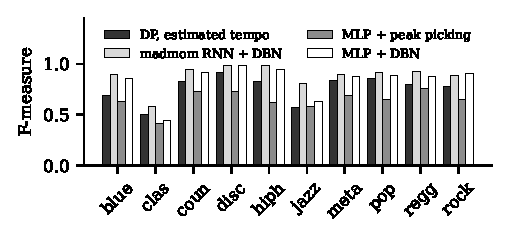
\includegraphics[width=\columnwidth]{../figures/fig_genre_f.pdf}
\caption{Mean beat F-measure per genre.}
\label{fig:genre}
\end{figure}

\begin{figure}[t]
\centering
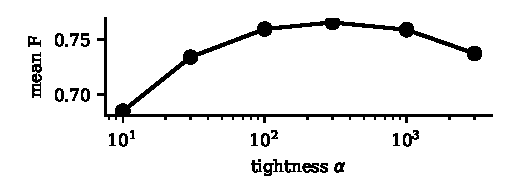
\includegraphics[width=\columnwidth]{../figures/fig_tightness.pdf}
\caption{Effect of the tightness $\alpha$ on the DP tracker with estimated tempo.}
\label{fig:tight}
\end{figure}

\section{Individual Status Report: Nalluraj Babu}
\label{sec:me}

\textbf{Objective 1: dynamic programming beat tracker.}
\emph{PI1 (basic, done).} The tracker takes the shared onset envelope and my own implementation of the tempo step of \cite{ellis}. This tempo estimate reaches Acc1 61\% and Acc2 90\% on the test split, against 70\% and 88\% for librosa's tempo.
\emph{PI2 (basic, done).} The DP recursion of Eq.~(\ref{eq:dp}) with backtracking runs in \DPTime{}\,s per minute of audio.
\emph{PI3 (expected, done).} Per genre (Figure~\ref{fig:genre}), disco, pop, country, hip-hop and metal are easy (F above 0.8), and classical (0.51) and jazz (0.58) are hard, because soft onsets and expressive timing give a weak and irregular envelope. The oracle tempo raises the mean F from \DPF{} to \DPOracleF{} and CMLt from \DPCML{} to \DPOracleCML{} (Table~\ref{tab:beats}). So a wrong tempo, mostly a wrong octave, is behind about two thirds of the CMLt errors, while beat placement itself is good.
\emph{PI4 (expected, done).} Given librosa's onset envelope and tempo, my tracker and librosa's agree at a median F of \AgreeRawMed{}; after adding the Gaussian smoothing that librosa applies to the envelope, the median is \AgreeMed{}, and \AgreeShare{}\% of the clips reach F $\ge 0.95$ against each other. Against the annotations, librosa (\LibF{}) and my tracker (\DPF{}) are equally accurate, and librosa is faster (\LibBeatTime{} against \DPTime{}\,s per minute). madmom is clearly better (F = \MadF{}, CMLt = \MadCML{}) but much slower; on our cloud machine it needs about \MadTime{}\,s per minute of audio. The tightness sweep (Figure~\ref{fig:tight}) has a flat optimum between 100 and 1000 (best $\alpha$ = \BestTight{}); very loose settings follow single onsets and very strict ones cannot recover from a slightly wrong period.
\emph{PI5 (advanced, not started).} Tempo following is planned for week 6.

\begin{figure}[t]
\centering
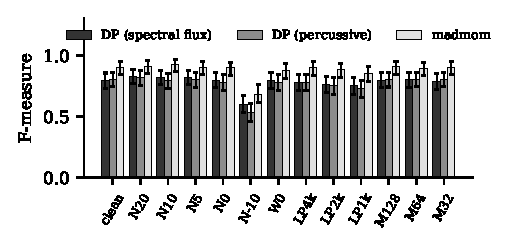
\includegraphics[width=\columnwidth]{../figures/fig_degradation.pdf}
\caption{Mean beat F-measure under degradation (\NDeg{} clips, estimated tempo): pink noise (N, SNR in dB), white noise (W0), low pass filter (LP) and MP3 bit rate (M).}
\label{fig:deg}
\end{figure}

\textbf{Objective 2: beat tracking on degraded audio.}
\emph{PI1 (basic, done).} \NDeg{} test clips were degraded in 13 conditions (Section~\ref{sec:methods}), using fixed random seeds so that every system sees the same audio.
\emph{PI2 (basic, done).} Figure~\ref{fig:deg} shows the F-measure of my tracker. MP3 down to 32\,kbps changes almost nothing (\DegMPThree{} against \DegClean{} clean). Low pass filtering hurts step by step, down to \DegLPOne{} at 1\,kHz, probably because the filter removes the attack of hi-hats and snares. Against our hypothesis, pink noise down to 0\,dB SNR does not lower the score (\DegNoiseZero{}), and white noise at 0\,dB also leaves it at \DegWhite{}. Only at $-10$\,dB does the score drop clearly, to \DegNoiseMinusTen{}. Stationary noise adds a constant floor to every band; after log compression this floor hides small fluctuations while strong drum onsets still rise above it, so the envelope can even get cleaner. With the oracle tempo the same pattern holds (\DegOrClean{} clean, \DegOrLPOne{} at 1\,kHz, \DegOrNoiseMinusTen{} at $-10$\,dB).
\emph{PI3 (expected, partly done).} madmom starts from \MadDegClean{} on these clips and falls to \MadDegLPOne{} at 1\,kHz and \MadDegNoiseMinusTen{} at $-10$\,dB, so the neural tracker is also hurt most by heavy noise and low pass filtering. At $-10$\,dB both lose about 0.2 in F, so madmom keeps its lead but is not more robust in relative terms. The 1D State Space tracker \cite{heydari} still has to be added.
\emph{PI4 (expected, done, negative result).} The percussive envelope gives \PercClean{} on clean audio but \PercLPOne{} at 1\,kHz and \PercNoiseMinusTen{} at $-10$\,dB, so it is never better than the plain spectral flux. Harmonic-percussive separation relies on the broadband shape of drum hits, which low pass filtering removes and loud noise covers.
\emph{PI5 (advanced, not started).} The plan is to set $\alpha$ from the peakiness of the onset envelope, using a loose tracker for strong, regular envelopes and a strict one for weak envelopes.

\textbf{What I learned and what did not work.} The DP tracker is accurate when it gets the right tempo, so most of its errors come from the tempo step. My expectation that noise would hurt most was wrong for our front end: bandwidth matters more than noise, and only very loud noise breaks the tracker. The percussive envelope did not help; a flux limited to the low bands, which survive low pass filtering, is the next thing to try.

\section{Team Status}
\label{sec:team}

\textbf{Irai Kumaran Sivanesan} built the autocorrelation tempo estimator. A simple octave decision raises Accuracy1 from \AccOneAC{}\% to \AccOnePrior{}\%, close to librosa (\AccOneLibrosa{}\%) and below madmom (\AccOneMadmom{}\%), while a pulse train stage did not help. His estimator is stable on time-stretched clips, and a sliding-window version with an octave-folded change detector finds a sudden tempo change within 2\,s in \DetFoldTwo{}\% of spliced clips. GiantSteps remains.

\textbf{Usha Sundaresan Manivannan} built a frame-wise neural network (an MLP on stacked log-mel features) and a low-frequency downbeat finder. The MLP reaches F = \NNF{} with peak picking and \NNDBNF{} with madmom's DBN decoder on its own activation (Table~\ref{tab:beats}). Her downbeat finder reaches \DBOracle{} on annotated beats against \DBMadBar{} for madmom's bar tracker on the same beats. The TCN in PyTorch and the advanced goals remain.

\PITable
\TimelineTable

\section{Revised Plan and Goals}

Our original plan assumed librosa, madmom and PyTorch from the start. Our first setup only had NumPy, SciPy and scikit-learn, so we built everything ourselves and moved the library comparisons later; these are now done for all three methods. Table~\ref{tab:pi} gives the status of every PI and Table~\ref{tab:time} the revised timeline.

\textbf{My goals for the final report.}
\emph{Basic:} keep the current tracker and degradation results, and extend the degradation study to all \NBeat{} test clips.
\emph{Expected:} add the 1D State Space tracker \cite{heydari} to the beat comparison and the degradation study, and try a low-band onset envelope for low pass filtered audio.
\emph{Advanced:} tempo following by letting the period change slowly along the DP path, evaluated on Irai's spliced clips, and an automatic choice of $\alpha$ from the onset envelope.

\textbf{Team goals.} Basic: every method and study complete on GTZAN. Expected: the TCN, the 1D State Space tracker in all comparisons, and GiantSteps. Advanced: tempo change detection on real music and a TCN with a downbeat output.

\section{Conclusion}

The dynamic programming tracker matches librosa in accuracy and behaviour and reaches \DPOracleF{} when the tempo is right. Under degradation it is robust to MP3 compression and moderate noise and loses most with strong low pass filtering and very loud noise, like madmom. The next steps are the 1D State Space comparison, a more robust envelope and the advanced goals.

\begin{thebibliography}{99}\small\setlength{\itemsep}{0pt}
\bibitem{tutorial} M. E. P. Davies, S. B\"ock, and M. Fuentes, ``Tempo, beat and downbeat estimation,'' Tutorial at ISMIR, 2021. [Online]. Available: https://tempobeatdownbeat.github.io/tutorial
\bibitem{bello} J. P. Bello, L. Daudet, S. Abdallah, C. Duxbury, M. Davies, and M. Sandler, ``A tutorial on onset detection in music signals,'' \emph{IEEE Trans. Speech Audio Process.}, vol. 13, no. 5, pp. 1035--1047, 2005.
\bibitem{gouyon} F. Gouyon, A. Klapuri, S. Dixon, M. Alonso, G. Tzanetakis, C. Uhle, and P. Cano, ``An experimental comparison of audio tempo induction algorithms,'' \emph{IEEE Trans. Audio, Speech, Lang. Process.}, vol. 14, no. 5, pp. 1832--1844, 2006.
\bibitem{percival} G. Percival and G. Tzanetakis, ``Streamlined tempo estimation based on autocorrelation and cross-correlation with pulses,'' \emph{IEEE/ACM Trans. Audio, Speech, Lang. Process.}, vol. 22, no. 12, pp. 1765--1776, 2014.
\bibitem{ellis} D. P. W. Ellis, ``Beat tracking by dynamic programming,'' \emph{J. New Music Res.}, vol. 36, no. 1, pp. 51--60, 2007.
\bibitem{librosa} B. McFee, C. Raffel, D. Liang, D. P. W. Ellis, M. McVicar, E. Battenberg, and O. Nieto, ``librosa: Audio and music signal analysis in Python,'' in \emph{Proc. Python in Science Conf. (SciPy)}, pp. 18--25, 2015.
\bibitem{plp} P. Grosche and M. M\"uller, ``Extracting predominant local pulse information from music recordings,'' \emph{IEEE Trans. Audio, Speech, Lang. Process.}, vol. 19, no. 6, pp. 1688--1701, 2011.
\bibitem{downbeat} S. B\"ock, F. Krebs, and G. Widmer, ``Joint beat and downbeat tracking with recurrent neural networks,'' in \emph{Proc. ISMIR}, 2016.
\bibitem{madmom} S. B\"ock, F. Korzeniowski, J. Schl\"uter, F. Krebs, and G. Widmer, ``madmom: A new Python audio and music signal processing library,'' in \emph{Proc. ACM Multimedia}, pp. 1174--1178, 2016.
\bibitem{krebsbar} F. Krebs, S. B\"ock, M. Dorfer, and G. Widmer, ``Downbeat tracking using beat-synchronous features and recurrent neural networks,'' in \emph{Proc. ISMIR}, 2016.
\bibitem{tcn} M. E. P. Davies and S. B\"ock, ``Temporal convolutional networks for musical audio beat tracking,'' in \emph{Proc. EUSIPCO}, 2019.
\bibitem{heydari} M. Heydari, M. McCallum, A. Ehmann, and Z. Duan, ``A novel 1D state space for efficient music rhythmic analysis,'' in \emph{Proc. ICASSP}, 2022.
\bibitem{degradation} M. Mauch and S. Ewert, ``The Audio Degradation Toolbox and its application to robustness evaluation,'' in \emph{Proc. ISMIR}, pp. 83--88, 2013.
\bibitem{daviseval} M. E. P. Davies, N. Degara, and M. D. Plumbley, ``Evaluation methods for musical audio beat tracking algorithms,'' Queen Mary Univ. of London, Tech. Rep. C4DM-TR-09-06, 2009.
\bibitem{mireval} C. Raffel, B. McFee, E. J. Humphrey, J. Salamon, O. Nieto, D. Liang, and D. P. W. Ellis, ``mir\_eval: A transparent implementation of common MIR metrics,'' in \emph{Proc. ISMIR}, 2014.
\bibitem{gtzan} G. Tzanetakis and P. Cook, ``Musical genre classification of audio signals,'' \emph{IEEE Trans. Speech Audio Process.}, vol. 10, no. 5, pp. 293--302, 2002.
\bibitem{sturm} B. L. Sturm, ``The GTZAN dataset: Its contents, its faults, their effects on evaluation, and its future use,'' arXiv:1306.1461, 2013.
\bibitem{kereliuk} C. Kereliuk, B. L. Sturm, and J. Larsen, ``Deep learning and music adversaries,'' \emph{IEEE Trans. Multimedia}, vol. 17, pp. 2059--2072, 2015.
\bibitem{marchand} U. Marchand, Q. Fresnel, and G. Peeters, ``GTZAN-Rhythm: Extending the GTZAN test-set with beat, downbeat and swing annotations,'' in \emph{Late-Breaking Demo, ISMIR}, 2015.
\bibitem{giantsteps} P. Knees, \'A. Faraldo, P. Herrera, R. Vogl, S. B\"ock, F. H\"orschl\"ager, and M. Le Goff, ``Two data sets for tempo estimation and key detection in electronic dance music annotated from user corrections,'' in \emph{Proc. ISMIR}, 2015.
\end{thebibliography}

\end{document}
